\chapter{Julia}

\say{\textsf{Julia} es un lenguaje de programación gratis y de código abierto desarrollado por Jeff Bezanson, Alan Edelman, Viral B. Shan y Stefan Karpinski en el MIT}, \cite{Hackers}.  Su propósito general es ser tan rápido como \textsf{C}, mientras mantiene la facilidad de lenguaje de \textsf{R} o \textsf{Python}. Es una combinación de sintaxis simple con alto rendimiento computacional. Su slogan es \say{\textsf{Julia} se ve como \textsf{Python}, se siente como \textsf{Lisp}, corre como \textsf{Fortran}}, \cite{Hackers}. 
Esta combinación de características hace que \textsf{Julia} sea un lenguaje de programación que ha tomado mucha fuerza  en la comunidad científica últimamente. Ya que es un lenguaje poco conocido, en esta sección se explica como instalar \textsf{Julia} en una computadora con sistema operativo \textsf{Windows} y algunos de los básicos del lenguaje.

\section{Reproducibilidad}
Antes de empezar, se enfatiza que esta tesis es completamente reproducible. Peng y Hicks del departamento de bioestadística en la Universidad John Hopkins definen \say{un análisis de datos publicado es reproducible si el conjunto de datos y el código utilizados para crear el análisis de datos está disponible para que otros lo analicen y estudien de manera independiente}, \cite{peng2021reproducible}. A pesar de que en el artículo enfatizan que esta definición puede ser un tanto ambigua, sí resaltan que la reproducibilidad es un medio para revisar y, posteriormente, confiar en el análisis de otros. 

Uno de los beneficios de tener un trabajo de investigación reproducible es que \say{los lectores obtienen los datos y el código computacional, los cuales son valiosos al grado de que pueden ser reutilizados o rediseñados para futuros estudios o investigaciones} \cite{peng2021reproducible}. El código programado para esta tesis se encuentra en la plataforma de GitHub, específicamente en la liga \url{https://github.com/valperez/Tesis_Julia}. Los datos utilizados también se pueden encontrar en la liga anterior o en la fuente que se indica al mencionarlos. 

\section{Instalación}
Este trabajo se presenta como si fuera hecho en un ambiente de \textsf{Windows}. La instalación y uso en los sistemas \textsf{Mac} y \textsf{Linux} es muy similar y no se mencionará.  

Al momento de la escritura de esta tesis la versión de \textsf{Julia} disponible es la \textsf{v1.6.3}. El primer paso es descargar \textsf{Julia} desde la página \url{https://julialang.org/downloads/}. 

Para el sistema operativo \textsf{Windows} se tiene la opción de un instalador de 64-bits o uno de 32-bits. El tipo de sistema que tiene un ordenador se verifica en \textsf{Start} $>$ \textsf{Configuración} $>$ \textsf{Sistema} $>$ \textsf{Acerca de}. Se debe seleccionar el \textsf{installer} y no el \textsf{portable}. Una vez descargado, se debe seleccionar el archivo \textsf{.exe} y seguir los pasos de instalación. 

\section{Símbolo del sistema}
Una vez instalado, se puede ejecutar \textsf{Julia} desde el símbolo del sistema o desde alguna interfaz gráfica como \textsf{Atom}, \textsf{Visual Studio Code} o \textsf{Jupyter Notebook}. De este último se explica más en el capítulo \ref{cap_jupyter}. 

Una de las ventajas de utilizar \textsf{Julia} desde el símbolo del sistema (también conocido como \textit{Command Prompt} o \texttt{cmd}) es que se pueden controlar algunos parámetros del lenguaje. Mi sugerencia es que se comience a usar \textsf{Julia} directo desde la interfaz nativa. Posteriormente, cuando se entienda lo básico y los programas generados requieran un mayor nivel computacional entonces se puede migrar a usar el \texttt{cmd} para correr \textsf{Julia}. 

\subsection{\textit{Multithreading}}
Una de las razones por la que \textsf{Julia} tiene gran velocidad es por su capacidad para multihilo (\textit{multithreading} en inglés). Esto significa que puede correr diferentes tareas de manera simultánea en varios hilos. Esto se debe a que la meta de los autores de \textsf{Julia} fue crear un lenguaje de programación con un rendimiento tan alto que pudiera hacer varias cosas simultáneamente. Debido a que uno de los objetivos de esta tesis es mostrar la eficiencia y velocidad de \textsf{Julia}, es crucial conocer la característica del \textit{multithreading} y cómo utilizarla. 

Si se está ejecutando \textsf{Julia} por medio del \texttt{cmd} es necesario modificar la cantidad de hilos que se va a utilizar antes de ejecutar \textsf{Julia}.  En \textsf{Windows}, esto se modifica programando \texttt{set Julia\_NUM\_THREADS=4} \citep{manual_Julia}. Si se está trabajando con otro sistema operativo, esta página puede ser una guía para modificar la cantidad de hilos \url{https://docs.julialang.org/en/v1/manual/multi-threading/}. En este ejemplo, se cambiaron los hilos a 4, pero se puede asignar cualquier número. Sin embargo, se recomienda que éste no exceda de la cantidad de procesadores lógicos de la computadora.  

Si se está usando \textsf{Julia} en algún editor de texto o programa externo la modificación del número de hilos se hace de forma diferente. Cada programa tiene su manera de hacerlo y usualmente las instrucciones vienen en el manual del mismo. Para observar que el cambio se ejecutó de manera correcta (independientemente de la opción elegida) basta con correr el comando \texttt{Threads.nthreads()} y observar que la respuesta sea el número deseado. 

\section{Básicos de Julia}
\say{Como el compilador de \textsf{Julia} es diferente a los intérpretes usados para lenguajes como \textsf{Python} o \textsf{R} se puede percibir que el funcionamiento de \textsf{Julia} no es intuitivo en un principio. Una vez que se entienda como funciona \textsf{Julia}, es fácil escribir código que es casi tan rápido como \textsf{C}}, \cite{manual_Julia}. En esta sección se da una introducción a la sintaxis del lenguaje que se tomó del manual oficial de \textsf{Julia}, \cite{manual_Julia}. 

La asignación de variables se hace con un signo de igualdad $=$. El ejemplo más sencillo de esto es ejecutar 
\begin{minted}{julia}
	julia> x = 2
	2
\end{minted}

\noindent donde se asigna a x el valor de 2. 

\subsection{Operaciones básicas}
La tabla \ref{operaciones_basicas_julia} muestra la sintaxis usada para las operaciones básicas en \textsf{Julia}. 

\begin{center}
	\begin{tabular}{|c|c|c|} 
		\hline
		Expresión & Nombre & Descripción \\ 
		\hline 
		\texttt{+x} & suma unaria & la operación identidad \\ 

		\texttt{-x} & resta unaria & asigna a los valores sus inversos aditivos \\ 

		\texttt{x + y} & suma binaria & realiza adición \\ 

		\texttt{x - y} & resta binaria & realiza sustracción \\

		\texttt{x * y} & multiplicación & realiza multiplicación \\

		\texttt{x / y} & división & realiza divisiones \\

		\texttt{x $\div$ y} & división de enteros & $x / y$ truncado a un entero \\

		\texttt{x $\setminus$ y} & división inversa & equivalente a dividir \texttt{y / x} \\

		\texttt{x $\wedge$ y} & potencia & eleva \texttt{x} a la potencia \texttt{y} \\

		\texttt{x \% y} & residuo & equivalente a \texttt{rem(x,y)} \\
		
		\texttt{!x} & negación & realiza lo contrario de \texttt{x} \\
		
		\texttt{x \& \& y} & \textit{and} lógico & verifica si \texttt{x} y \texttt{y} se cumplen \\
		
		\texttt{x || y} & \textit{or} lógico & verifica si al menos uno, \texttt{x} o \texttt{y},  se cumplen \\
		\hline
	\end{tabular} 
	\captionof{table}{Operaciones básicas en Julia} \label{operaciones_basicas_julia}
\end{center}


\subsubsection{Operaciones básicas en vectores}
En \textsf{Julia} cada operación binaria tiene su correspondiente operación punto (\textit{dot operation} en inglés). Estas funciones están definidas para efectuarse elemento por elemento en vectores y matrices. Para llamarse basta agregar un punto antes del operador binario. Por ejemplo,

\begin{minted}{julia}
	julia> [1 9 9 7] .^ 2
	1x4 Matrix{Int64}:
	1 81 81 49
\end{minted}

 \noindent eleva cada uno de los elementos del vector al cuadrado. 

\textsf{Julia} maneja los números imaginarios utilizando el sufijo \texttt{im}. Sin embargo, no se utilizaron en este trabajo así que se omitirá dar mayor explicación. 

\subsection{\textit{Strings} (secuencias de caracteres)} 

Además de números, \textsf{Julia} puede asignar una secuencia de caracteres (mejor conocido como string) a variables usando comillas dobles. Se puede accesar a caracteres específicos de un string utilizando corchetes cuadrados $[$ $]$ y a cadenas seguidas de caracteres usando dos puntos $:$. Por ejemplo,

\begin{minted}{julia}
    julia> string = "Esta tesis es interesante"
    julia> string[6]
    't': ASCII/Unicode U+0074 (category Ll: Letter, lowercase)
    
    julia> string[4:8]
    "a tes"
\end{minted}

Además, \textsf{Julia} también tiene la opción de concatenación de múltiples strings. Esto se hace utilizando un asterisco $*$ para separar cada uno de los strings. Por ejemplo,

\begin{minted}{julia}
	julia> grado = "licenciada"
	julia> nexo = "en"
	julia> carrera = "matematicas aplicadas"
	julia> espacio = " "
	julia> grado*espacio*nexo*espacio*carrera
	"licenciada en matematicas aplicadas"
\end{minted}

\subsection{Funciones}
En \textsf{Julia} una función es un objeto que asigna una tupla de argumentos a un valor de retorno \cite{manual_Julia}. La sintáxis básica para definir funciones en \textsf{Julia} es 

\begin{minted}{julia}
	julia> function suma(x, y)
		x + y
	end
\end{minted}

Además, se puede agregar la palabra \texttt{return} para que la función regrese un valor. Por ejemplo, si se quisiera tener una función a la que se le dan dos números y regrese el número mayor, los comandos serian de la forma:

\begin{minted}{julia}
	julia> function numero_mayor(x, y)
		if (x > y)
			return x
		else
			return y
		end
	end
\end{minted}


Para llamar a la función basta con escribir \texttt{numero\_mayor(x, y)} asignando o sustituyendo valores por $x$ y $y$. Por ejemplo,

\begin{minted}{julia}
	julia> numero_mayor(4, 9)
	9
	
\end{minted}

\subsection{Vectores y Matrices}

Un vector columna de $n$ componentes se define como un conjunto ordenado de $n$ números escritos de la siguiente manera:
\begin{equation*}
    \begin{aligned}
    \begin{pmatrix}
    x_1 \\ 
    x_2 \\
    \vdots \\
    x_n
    \end{pmatrix} 
    \end{aligned}
\end{equation*}

En \textsf{Julia} para definir un vector columna se hace uso de los corchetes cuadrados $[$ $]$ y comas. Por ejemplo, 

\begin{minted}{julia}
	julia> A = [1, 9, 9, 7]
	4-element Vector{Int64}
	1
	9
	9
	7
\end{minted}

\noindent da como resultado un vector de 4 elementos de tipo Int64. \textsf{Julia} es un lenguaje exigente con los tipos de objetos, por lo que aprender sus características y funciones singulares es uno de los atributos que hacen a un buen usuario. 

Si se quisiera definir un vector renglón se haría exactamente lo mismo excepto que se omitiría el uso de las comas. En este caso, \textsf{Julia} tomó el objeto \texttt{A} como una matriz, no como un vector. 

Una matriz $A$ de $m \times n$ es un arreglo rectangular de $mn$ números dispuestos en $m$ renglones y $n$ columnas. 

\begin{equation*}
    \begin{aligned}
    \begin{pmatrix}
    a_{11} & a_{12} & \dots & a_{1j} & \dots & a_{1n} \\
    a_{21} & a_{22} & \dots & a_{2j} & \dots & a_{2n} \\
    \vdots &  \vdots  &  \ddots &  \vdots  & \ddots &\vdots\\
    a_{i1} & a_{i2} & \dots & a_{ij} & \dots & a_{in} \\
    \vdots &  \vdots  &  \ddots &  \vdots  & \ddots &\vdots\\
     a_{m1} & a_{m2} & \dots & a_{mj} & \dots & a_{mn} \\
    \end{pmatrix} 
    \end{aligned}
\end{equation*}

En \textsf{Julia}, hay dos formas de definir matrices. La primera es utilizando los corchetes cuadrados $[$ $]$ para comenzar y terminar la matriz. Las columnas están separadas por espacios y las filas por punto y coma. La segunda opción es similar a la primera con la única diferencia de que en lugar de punto y coma se cambia de renglón. Esta opción puede parecer tediosa ya que requiere que las columnas estén alineadas. Sin embargo, es una forma más visual de ver las matrices. Lo siguientes comandos muestran ambas opciones. 

\begin{minted}{julia}
	julia> A_1 = [1 2 3; 4 5 6]
	2x3 Matrix{Int64}
	1 2 3
	4 5 6
	julia> A_2 = [1 2 3
		      4 5 6]
	2x3 Matrix{Int64}
	1 2 3
	4 5 6

\end{minted}

De manera análoga con los vectores, para llamar un solo elemento de la matriz se utilizan los corchetes cuadrados. Continuando con el ejemplo anterior, para obtener el número 5 de la matriz $\texttt{A\_2}$, se introduciría el comando 
\begin{minted}{julia}
	julia> A_2[2, 2]
	5
\end{minted}

\textsf{Julia} necesita de la instalación del paquete \textsf{LinearAlgebra} para hacer operaciones básicas y factorización de matrices. El catálogo de funciones es bastante extenso para incluirlo en este trabajo, pero se puede encontrar en \url{https://docs.julialang.org/en/v1/stdlib/LinearAlgebra/}.

\subsection{Instalación de un paquete} \label{instalacion_paquete}


Para cualquier otra operación fuera de lo básico que ya se mencionó, \textsf{Julia} necesita usar paquetes. Los paquetes son similar a las librerías en \textsf{R}. La lista completa de paquetes registrados en \textsf{Julia} se encuentra en \url{https://juliapackages.com/}. En esta sección se explica la instalación y uso de los mismos. 

El único paquete que ya viene por default en la instalación de \textsf{Julia} es \texttt{Pkg} ya que su función es instalar otros paquetes. El comando \texttt{using} activa un paquete ya descargado mientras que \texttt{Pkg.add()} agrega un paquete nuevo. A continuación se presenta la guía básica para descargar cualquier paquete en \textsf{Julia} usando como ejemplo al ya mencionado \texttt{LinearAlgebra}. 


\begin{minted}{julia}
	using Pkg
	Pkg.add("LinearAlgebra")
	using LinearAlgebra
\end{minted}

La instalación de un paquete solo se debe hacer una vez. Si se requiere usar en alguna sesión posterior basta con usar el comando \texttt{using} y el nombre del paquete. En las siguientes secciones se explica y ejemplifica el uso de dos paquetes muy usados en esta tesis. 

\subsection{\textit{DataFrames}}

Un \textit{dataframe} es una tabla estructurada de dos dimensiones que se usa para tabular distintos tipos de datos. \textsf{Julia} tiene un paquete llamado \texttt{DataFrames} que permite trabajar con dataframes de creación propia o de alguna fuente externa. 

\subsubsection{Crear un dataframe}

Los dataframes pueden ser usados para manejar grandes cantidades de información exportada o pueden ser creaciones propias en el lenguaje. Para crear un dataframe desde cero en \textsf{Julia} se debe escribir la palabra \texttt{DataFrame} y abrir un paréntesis. Después, se escribe el nombre de la primera columna, un signo de igualdad y los datos que corresponden a esa variable. Se repite lo mismo con la cantidad de columnas que se requieran. Por ejemplo, para hacer un dataframe con las claves únicas y nombres de cinco mujeres el código sería el siguiente: 


\begin{minted}{julia}
	julia> using DataFrames
	julia> df = DataFrame(id = 1:5, 
   			nombre = ["Valeria", "Paula", 
   			"María José", "Sofía", "Mónica"])
\end{minted}

Los nombres de las columnas de un dataframe se vuelven una especie de atributos. Para referirse a la columna 'col' del dataframe 'df' basta escribir \texttt{df.col}. Si se quisiera agregar una columna nueva se deben asignar datos a \texttt{df.colNueva}. Por ejemplo, si quisiera agregar una columna llamada \texttt{color} al dataframe del ejemplo anterior, el código sería el siguiente: 

\begin{minted}{julia}
     julia> df.color = ["morado", "azul", "verde", "negro", "rojo"]
\end{minted}

\subsubsection{Importar datos en un dataframe}

Como ya se mencionó, los dataframes son utilizados para contener grandes cantidades de información. Usualmente esta información no es generada en \textsf{Julia} por lo que hay importarla. Una de las formas más rápidas es usando el paquete \texttt{CSV}. La descarga de este paquete se hace siguiendo  los pasos descritos en la sección \ref{instalacion_paquete}. 

Una vez instalado el programa, se necesita utilizar el comando \texttt{CSV.read} y la ruta de la ubicación del archivo para exportar los datos. 

\begin{minted}{julia}
	julia> using CSV, DataFrames
        julia> df = CSV.read("~/ejemplo.csv", DataFrame)
\end{minted}

\begin{figure}[h]
\begin{center}
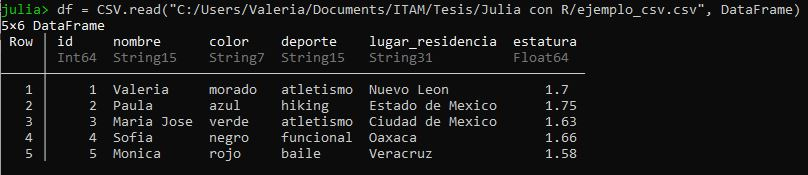
\includegraphics[scale=0.6]{Imagenes/insertar_df.PNG}
	\caption{Ejemplo de importación de un dataframe}
  \label{insertar_df}
\end{center}
\end{figure}

Los dataframes tienen una cantidad inmensa de funciones que incluyen agregar o eliminar información, seleccionar columnas o renglones, transformar su contenido, etc. Las especificaciones de dichas funciones se explican con mayor profundidad en el manual oficial del paquete en la página \url{https://dataframes.juliadata.org/stable/}. 

\subsection{Análisis de regresión} \label{cap_regresiones}

Un análisis de regresión es una herramienta estadística para estudiar las relaciones entre distintas variables. \say{Regresión es un método que permite a los investigadores resumir como predicciones o valores promedio de un resultado varían a través de variables individuales definidas como predictores o regresores}, \cite{regression_other_stories}. 

En distintas palabras, la regresión es una expresión que intenta explicar como una variable depende otras. En \textsf{Julia}, esto se puede hacer con ayuda del paquete \texttt{GLM}, ya que facilita el ajuste de modelos lineales. Como todos los paquetes, primero se debe instalar con los pasos descritos en \ref{instalacion_paquete}. 

En este paquete una de las funciones principales se llama \texttt{lm} que se utiliza para ajustar un modelo lineal a un conjunto de datos. En el manual oficial \cite{glm_manual} está descrita la manera en que se pueden generar modelos más avanzados. Esta función se utiliza en repetidas ocasiones en este trabajo por lo que se explica a continuación. La función es \texttt{lm(formula, data, allowrankdeficient=false; [wts::AbstractVector], dropcollinear::Bool=true)} donde 

\valinline{FALTA}

\begin{itemize}
    \item \texttt{formula}: usa los nombres de las columnas del dataframe de datos para referirse a las variables predictoras. Debe ser un objeto de tipo \texttt{formula}. 
    
    \item \texttt{data}: el dataframe que contenga los datos de los predictores de la fórmula.
    
    \item \texttt{allowrankdeficient}
    
    \item \texttt{wts}: es un vector que especifica la ponderación de las observaciones. 
    
    \item \texttt{dropcolliinear}: controla si \texttt{lm} acepta una matriz que no sea de rango completo. 
\end{itemize}



\subsubsection{Regresión lineal simple}
El modelo de regresión lineal más simple es el que tiene un solo predictor

\begin{equation*}
    \begin{aligned}
    y = a + bx + \epsilon
    \end{aligned}
\end{equation*}

Para ejemplificar este modelo de regresión se usaron los datos de \cite{regression_other_stories}. Dicha información fue recabada por Douglas Hibbs con el objetivo de predecir las elecciones de Estados Unidos basándose solamente en el crecimiento económico. Los datos se ven de la siguiente manera: 

\begin{figure}[H]
\begin{center}
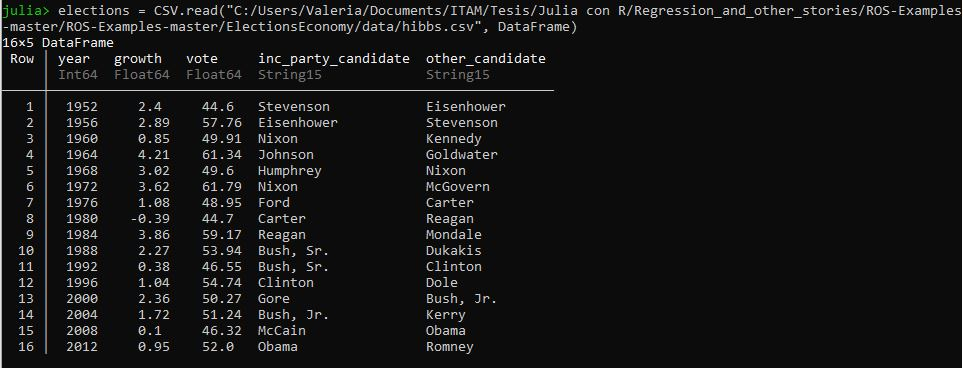
\includegraphics[scale=0.5]{Imagenes/elections_dataframe.PNG}
\caption{Encabezado de los datos sobre las elecciones en EUA recabados por Douglas Hibbs}
  \label{elections_dataframe}
\end{center}
\end{figure}

En este modelo se busca que el voto sea resultado del crecimiento económico. El código para hacer esto en \textsf{Julia} es

\begin{minted}{julia}
	elections_lm = lm(@formula(vote ~ growth), elections)
\end{minted}

El resultado es una tabla con los coeficientes, la desviación estándar, el valor \textit{t}, el valor$-p$ y el intervalo de confianza del $95 \% $ para los coeficientes. En este ejemplo, el resultado que da \textsf{Julia} es \texttt{y = 46.3 + 3.1x}, el cual coincide con los valores reportados en el libro.

\subsubsection{Regresión lineal múltiple}
La regresión lineal múltiple es el caso general de la regresión lineal simple. La diferencia es que en el primero hay múltiples predictores que deben cumplir ciertos criterios. \cite{regression_other_stories} define este tipo de regresión como 

\begin{equation*}
    \begin{aligned}
    y_i = \beta_1 X_{i1} + \dots + \beta_k X_{ik} + \epsilon_i, \text{ para } i = 1, \dots, n
    \end{aligned}
\end{equation*}

\noindent donde los errores $\epsilon_i$ son independientes e idénticamente distribuidos de manera normal con media 0 y varianza $\sigma^2$. La representación matricial equivalente es 

\begin{equation} \label{eq_rlm}
    \begin{aligned}
        y_i = X_i \beta + \epsilon_i, \text{ para } i = 1, \dots, n
    \end{aligned}
\end{equation}

\noindent donde $X$ es una matriz de $n \times k$ con renglón $X_i$.

Para ejemplificar este tipo de modelo se uso un ejemplo que consta de dos predictores y la interacción entre ellos. De nuevo se utilizaron los datos de \cite{regression_other_stories} que muestran la relación entre los resultados de exámenes de niños (\texttt{kid\_score}), el coeficiente intelectual IQ de sus madres (\texttt{mom\_iq}) y si sus madres terminaron o no la preparatoria (\texttt{mom\_hs}). 

Se buscó determinar si existe una relación significativa entre la educación y el coeficiente de las madres con los resultados de los exámenes de sus hijos. Por lo tanto, los predictores son las variables en relación con la madre mientras que la respuesta es el desempeño de los niños. El código en \textsf{Julia} se ve de la siguiente manera

\begin{minted}{julia}
    julia> using DataFrames, GLM, CSV
    julia> data_kid = CSV.read("~/Tesis/data/kidiq.csv", DataFrame)
    julia> fm = @formula(kid_score ~ mom_hs + mom_iq + mom_hs*mom_iq)
    julia> kidscore_lm = lm(fm, data_kid)
\end{minted}

Que da como resultado el modelo ajustado

\texttt{kid\_score = -11.48 + 51.26* mom\_hs + 0.97*mom\_iq - 0.48*mom\_hs*mom\_iq}

Uno de los aspectos por resaltar en este ejemplo es que para incluir la relación entre dos predictores se usa un asterisco entre ellos al momento de definir la fórmula de la regresión. 

En el caso donde alguno de los regresores sea de tipo categórico la fórmula se mantiene igual pero hay que hacerle cambios a la base de datos en sí. Si \textsf{Julia} no reconoce estas columnas como categóricas entonces se debe cambiar su tipo en el dataframe. Se aborda este problema más a fondo en el capítulo \ref{reg_categorias}. 

Por otro lado, se puede intentar usar el paquete \texttt{CSVFiles} para leer los archivos ya que hace mejor trabajo identificando el tipo de variables. Sin embargo, este paquete todavía está en desarrollo. 
